
%% bare_jrnl.tex
%% V1.3
%% 2007/01/11
%% by Michael Shell
%% see http://www.michaelshell.org/
%% for current contact information.
%%
%% This is a skeleton file demonstrating the use of IEEEtran.cls
%% (requires IEEEtran.cls version 1.7 or later) with an IEEE journal paper.
%%
%% Support sites:
%% http://www.michaelshell.org/tex/ieeetran/
%% http://www.ctan.org/tex-archive/macros/latex/contrib/IEEEtran/
%% and
%% http://www.ieee.org/



% *** Authors should verify (and, if needed, correct) their LaTeX system  ***
% *** with the testflow diagnostic prior to trusting their LaTeX platform ***
% *** with production work. IEEE's font choices can trigger bugs that do  ***
% *** not appear when using other class files.                            ***
% The testflow support page is at:
% http://www.michaelshell.org/tex/testflow/


%%*************************************************************************
%% Legal Notice:
%% This code is offered as-is without any warranty either expressed or
%% implied; without even the implied warranty of MERCHANTABILITY or
%% FITNESS FOR A PARTICULAR PURPOSE! 
%% User assumes all risk.
%% In no event shall IEEE or any contributor to this code be liable for
%% any damages or losses, including, but not limited to, incidental,
%% consequential, or any other damages, resulting from the use or misuse
%% of any information contained here.
%%
%% All comments are the opinions of their respective authors and are not
%% necessarily endorsed by the IEEE.
%%
%% This work is distributed under the LaTeX Project Public License (LPPL)
%% ( http://www.latex-project.org/ ) version 1.3, and may be freely used,
%% distributed and modified. A copy of the LPPL, version 1.3, is included
%% in the base LaTeX documentation of all distributions of LaTeX released
%% 2003/12/01 or later.
%% Retain all contribution notices and credits.
%% ** Modified files should be clearly indicated as such, including  **
%% ** renaming them and changing author support contact information. **
%%
%% File list of work: IEEEtran.cls, IEEEtran_HOWTO.pdf, bare_adv.tex,
%%                    bare_conf.tex, bare_jrnl.tex, bare_jrnl_compsoc.tex
%%*************************************************************************

% Note that the a4paper option is mainly intended so that authors in
% countries using A4 can easily print to A4 and see how their papers will
% look in print - the typesetting of the document will not typically be
% affected with changes in paper size (but the bottom and side margins will).
% Use the testflow package mentioned above to verify correct handling of
% both paper sizes by the user's LaTeX system.
%
% Also note that the "draftcls" or "draftclsnofoot", not "draft", option
% should be used if it is desired that the figures are to be displayed in
% draft mode.
%
\documentclass[journal]{IEEEtran}
\usepackage{blindtext}
\usepackage{graphicx}


\usepackage{cite}

\usepackage[cmex10]{amsmath}

\usepackage{url}


% correct bad hyphenation here
\hyphenation{}


\begin{document}

%
% paper title
% can use linebreaks \\ within to get better formatting as desired
\title{Will Millennials Ever Get Married?}
%
%
% author names and IEEE memberships
% note positions of commas and nonbreaking spaces ( ~ ) LaTeX will not break
% a structure at a ~ so this keeps an author's name from being broken across
% two lines.
% use \thanks{} to gain access to the first footnote area
% a separate \thanks must be used for each paragraph as LaTeX2e's \thanks
% was not built to handle multiple paragraphs
%

\author{Allen B. Downey% <-this % stops a space
\thanks{Olin College of Engineering, Needham MA 02492 USA e-mail: allen.downey@olin.edu}}





% The paper headers
%\markboth{}%
%{}
% The only time the second header will appear is for the odd numbered pages
% after the title page when using the twoside option.
% 
% *** Note that you probably will NOT want to include the author's ***
% *** name in the headers of peer review papers.                   ***
% You can use \ifCLASSOPTIONpeerreview for conditional compilation here if
% you desire.




% If you want to put a publisher's ID mark on the page you can do it like
% this:
%\IEEEpubid{0000--0000/00\$00.00~\copyright~2007 IEEE}
% Remember, if you use this you must call \IEEEpubidadjcol in the second
% column for its text to clear the IEEEpubid mark.



% use for special paper notices
%\IEEEspecialpapernotice{(Invited Paper)}




% make the title area
\maketitle


\begin{abstract}
%\boldmath
We investigate marriage patterns among women in the United States
with data from the National Survey of Family Growth (NSFG).
Using survival analysis methods implemented in Python, we
describe age at first marriage for successive cohorts based
on decade of birth.  Of women born in the 1980s,
60\% are married by age 32; of women born in 1990s, 13\%
are married by age 22.  For both groups these results reflect
substantial and statistically significant decreases compared to
previous cohorts.
\end{abstract}


% Note that keywords are not normally used for peerreview papers.
\begin{IEEEkeywords}
Survival analysis, marriage patterns.
\end{IEEEkeywords}






% For peer review papers, you can put extra information on the cover
% page as needed:
% \ifCLASSOPTIONpeerreview
% \begin{center} \bfseries EDICS Category: 3-BBND \end{center}
% \fi
%
% For peerreview papers, this IEEEtran command inserts a page break and
% creates the second title. It will be ignored for other modes.
%\IEEEpeerreviewmaketitle



\section{Introduction}

A recent study from the Pew Research Center\cite{wang14} reports that
the fraction of adults in the U.S.\ who have never married is increasing.
In 2012, 23\% of men 25 and older had never married, and
17\% of women.  In 1960, only 10\% of men were unmarried and 8\% of women.
Their report focuses on the causes of these trends, but does not
address this question: is the fraction of people who never marry
increasing, are people marrying later, or both?  That is the subject
of this paper.

To answer these questions, we apply tools of survival analysis to data
from the National Survey of Family Growth (NSFG).
Since 1973 the U.S.\ Centers for Disease Control and Prevention (CDC)
have conducted this survey, intended to gather ``information on family life, marriage and divorce, pregnancy, infertility, use of contraception, and men's
and women'shealth.'' See \url{http://cdc.gov/nchs/nsfg.htm}.

NSFG data is organized in cycles; during each cycle several thousand
respondents were interviewed, including women ages 14--44.  Men were
included starting with Cycle 6 in 2002, but for this study we use only
data from female respondents.

Table~\ref{tab:nsfg} shows the interview dates for each cycle, the
number of respondents, and the birth years of the respondents.
We did not use data from Cycles 1 and 2 because they included only
married women.  The total sample size for this study is 52 789.  

\begin{table}[h]
\centering
\begin{tabular}{c|c|r|c}
Cycle & Interview & Number of & Birth \\
       & Dates & Respondents  & Years \\
\hline
3 &  1982--83 & 7 969 & 1937--68 \\
4 &  1988--88 & 8 450 & 1943--73 \\
5 &  1995 & 10 847 & 1950--80 \\
6 &  2002--03 & 7 643 & 1957--88 \\
7 &  2006--10 & 12 279 & 1961--95 \\
8 &  2011--13 & 5 601 & 1966--98 \\
\end{tabular}
\caption{NSFG Survey Cycles}
\label{tab:nsfg}
\end{table}

For each respondent we have date of birth (year and month), date
of interview, and date of first marriage, if applicable.  So we can
compute with resolution of one month the respondent's age at
interview, {\tt age}, and age at first marriage, {\tt agemarry}.

To study changes in marriage patterns over time, we group the
respondents into cohorts by decade of birth.  For each cohort, 
Table~\ref{tab:cohorts} reports the number of respondents, range
of ages when they were interviewed, number who had been married at
least once at time of interview, and the number of married respondents
whose date of marriage was not ascertained.

Cohort 30
refers to women who born in the 1930s.  The focus of this
paper is to describe and predict marriage patterns of the
last two cohorts, women born in the 1980s and 90s.

\begin{table}[ht]
\centering
\begin{tabular}{c|r|c|r|r}
Cohort & Number of    & Age at     & Number  & Missing Age \\
       & Respondents  & Interview  & Married & at Marriage \\
\hline
30 & 325 & 42--44 & 310 & 0 \\
40 & 3 608 & 32--44 & 3275 & 0 \\
50 & 10 631 & 22--44 & 8658 & 10 \\
60 & 14 484 & 15--44 & 8421 & 27 \\
70 & 12 083 & 14--43 & 5908 & 25 \\
80 & 8 536 & 14--33 & 2203 & 8 \\
90 & 3 122 & 15--23 & 93 & 0 \\
\end{tabular}
\caption{NSFG Birth Cohorts}
\label{tab:cohorts}
\end{table}





\section{Methodology}


\subsection{Survival analysis}

Survival analysis is a powerful set of tools with applications in many
domains, but it is often considered a specialized topic.
One goal of this paper is to introduce survival analysis, using Python,
for people who are not already familiar with it.

Survival analysis is used to study and predict the time until an event: in
medicine, the event might be the death of a patient, hence ``survival'';
but more generally we might be interested in the time until failure
of a mechanical part, the lifetimes of civilizations, species, or
stars; or in this study the time from birth until first marriage.

The result of survival analysis is most often a {\bf survival function},
which shows the fraction of the population that survives after $t$,
for any time, $t$.  If $T$ is a random variable that represents the
time until an event, the survival function, $S(t)$, is the
probability that $T$ exceeds $t$:
%
\begin{equation}
S(t) \equiv \mathrm{Pr}(T > t)
\end{equation}
%
If the distribution of $T$ is known, or can be estimated from a
representative sample, computing $S(t)$ is simple: it is the
complement of the cumulative distribution function (CDF):
%
\begin{equation}
S(t) = 1 - \mathrm{CDF_T}(t)
\end{equation}
%
In Python we can compute the survival function like this:

\begin{verbatim}
from collections import Counter
import numpy as np

def MakeSurvivalFunction(values):
    counter = Counter(values)
    ts, fs = zip(*sorted(counter.items()))
    ts = np.asarray(ts)
    ps = np.cumsum(fs, dtype=np.float)
    ps /= ps[-1]
    ss = 1 - ps
    return SurvivalFunction(ts, ss)
\end{verbatim}

{\tt values} is a sequence of observed lifetimes.  {\tt Counter}
makes a map from each unique value to the number of times it
appears, which we split into a sorted sequence of times, {\tt ts}, and
their frequencies, {\tt fs}.

We convert {\tt ts} to a NumPy array (see \url{http://www.numpy.org/}).
Then {\tt ps} is the cumulative sum of
the frequencies, normalized to go from 0 to 1, so it represents
the CDF of the observed values.  {\tt ss}, which is the complement
of {\tt ps}, is the survival function.

{\tt SurvivalFunction} is defined in {\tt marriage.py},
a Python module we wrote for this project.  The code and data for this
project are available in a public Git repository at
\url{https://github.com/AllenDowney/MarriageNSFG}.

Given a survival curve, we can compute the {\bf hazard function},
which is the instantaneous death rate at time $t$; that is, the
fraction of people who survive until time $t$ and then die at time $t$.
When $t$ is continuous, the hazard function, $\lambda(t)$, is
%
\begin{equation}
\lambda(t) = -S'(t) / S(t)
\end{equation}
%
Where $S'(t)$ is the derivative of $S(t)$.  Since the survival
function decreases monotonically, its derivative is nonpositive,
so the hazard function is nonnegative.

With a survival function represented by discrete {\tt ts} and {\tt ss},
we can compute the hazard function like this:

\begin{verbatim}
import pandas as pd

# class SurvivalFunction
def MakeHazardFunction(self):
    lams = pd.Series(index=self.ts)
    prev = 1.0
    for t, s in zip(self.ts, self.ss):
        lams[t] = (prev - s) / prev
        prev = s
    return HazardFunction(lams)
\end{verbatim}

{\tt MakeHazardFunction} is a method of {\tt SurvivalFunction},
which provides attributes {\tt ts} and {\tt ss}.  The result,
{\tt lams}, is a Pandas Series object that maps from the
same set of {\tt ts} to the estimated hazard function, $\lambda(t)$
(see \url{http://pandas.pydata.org}).

%This result could be computed faster using {\tt np.diff}, but
%his version makes the computation more readable.

\begin{figure}[!t]
\centering
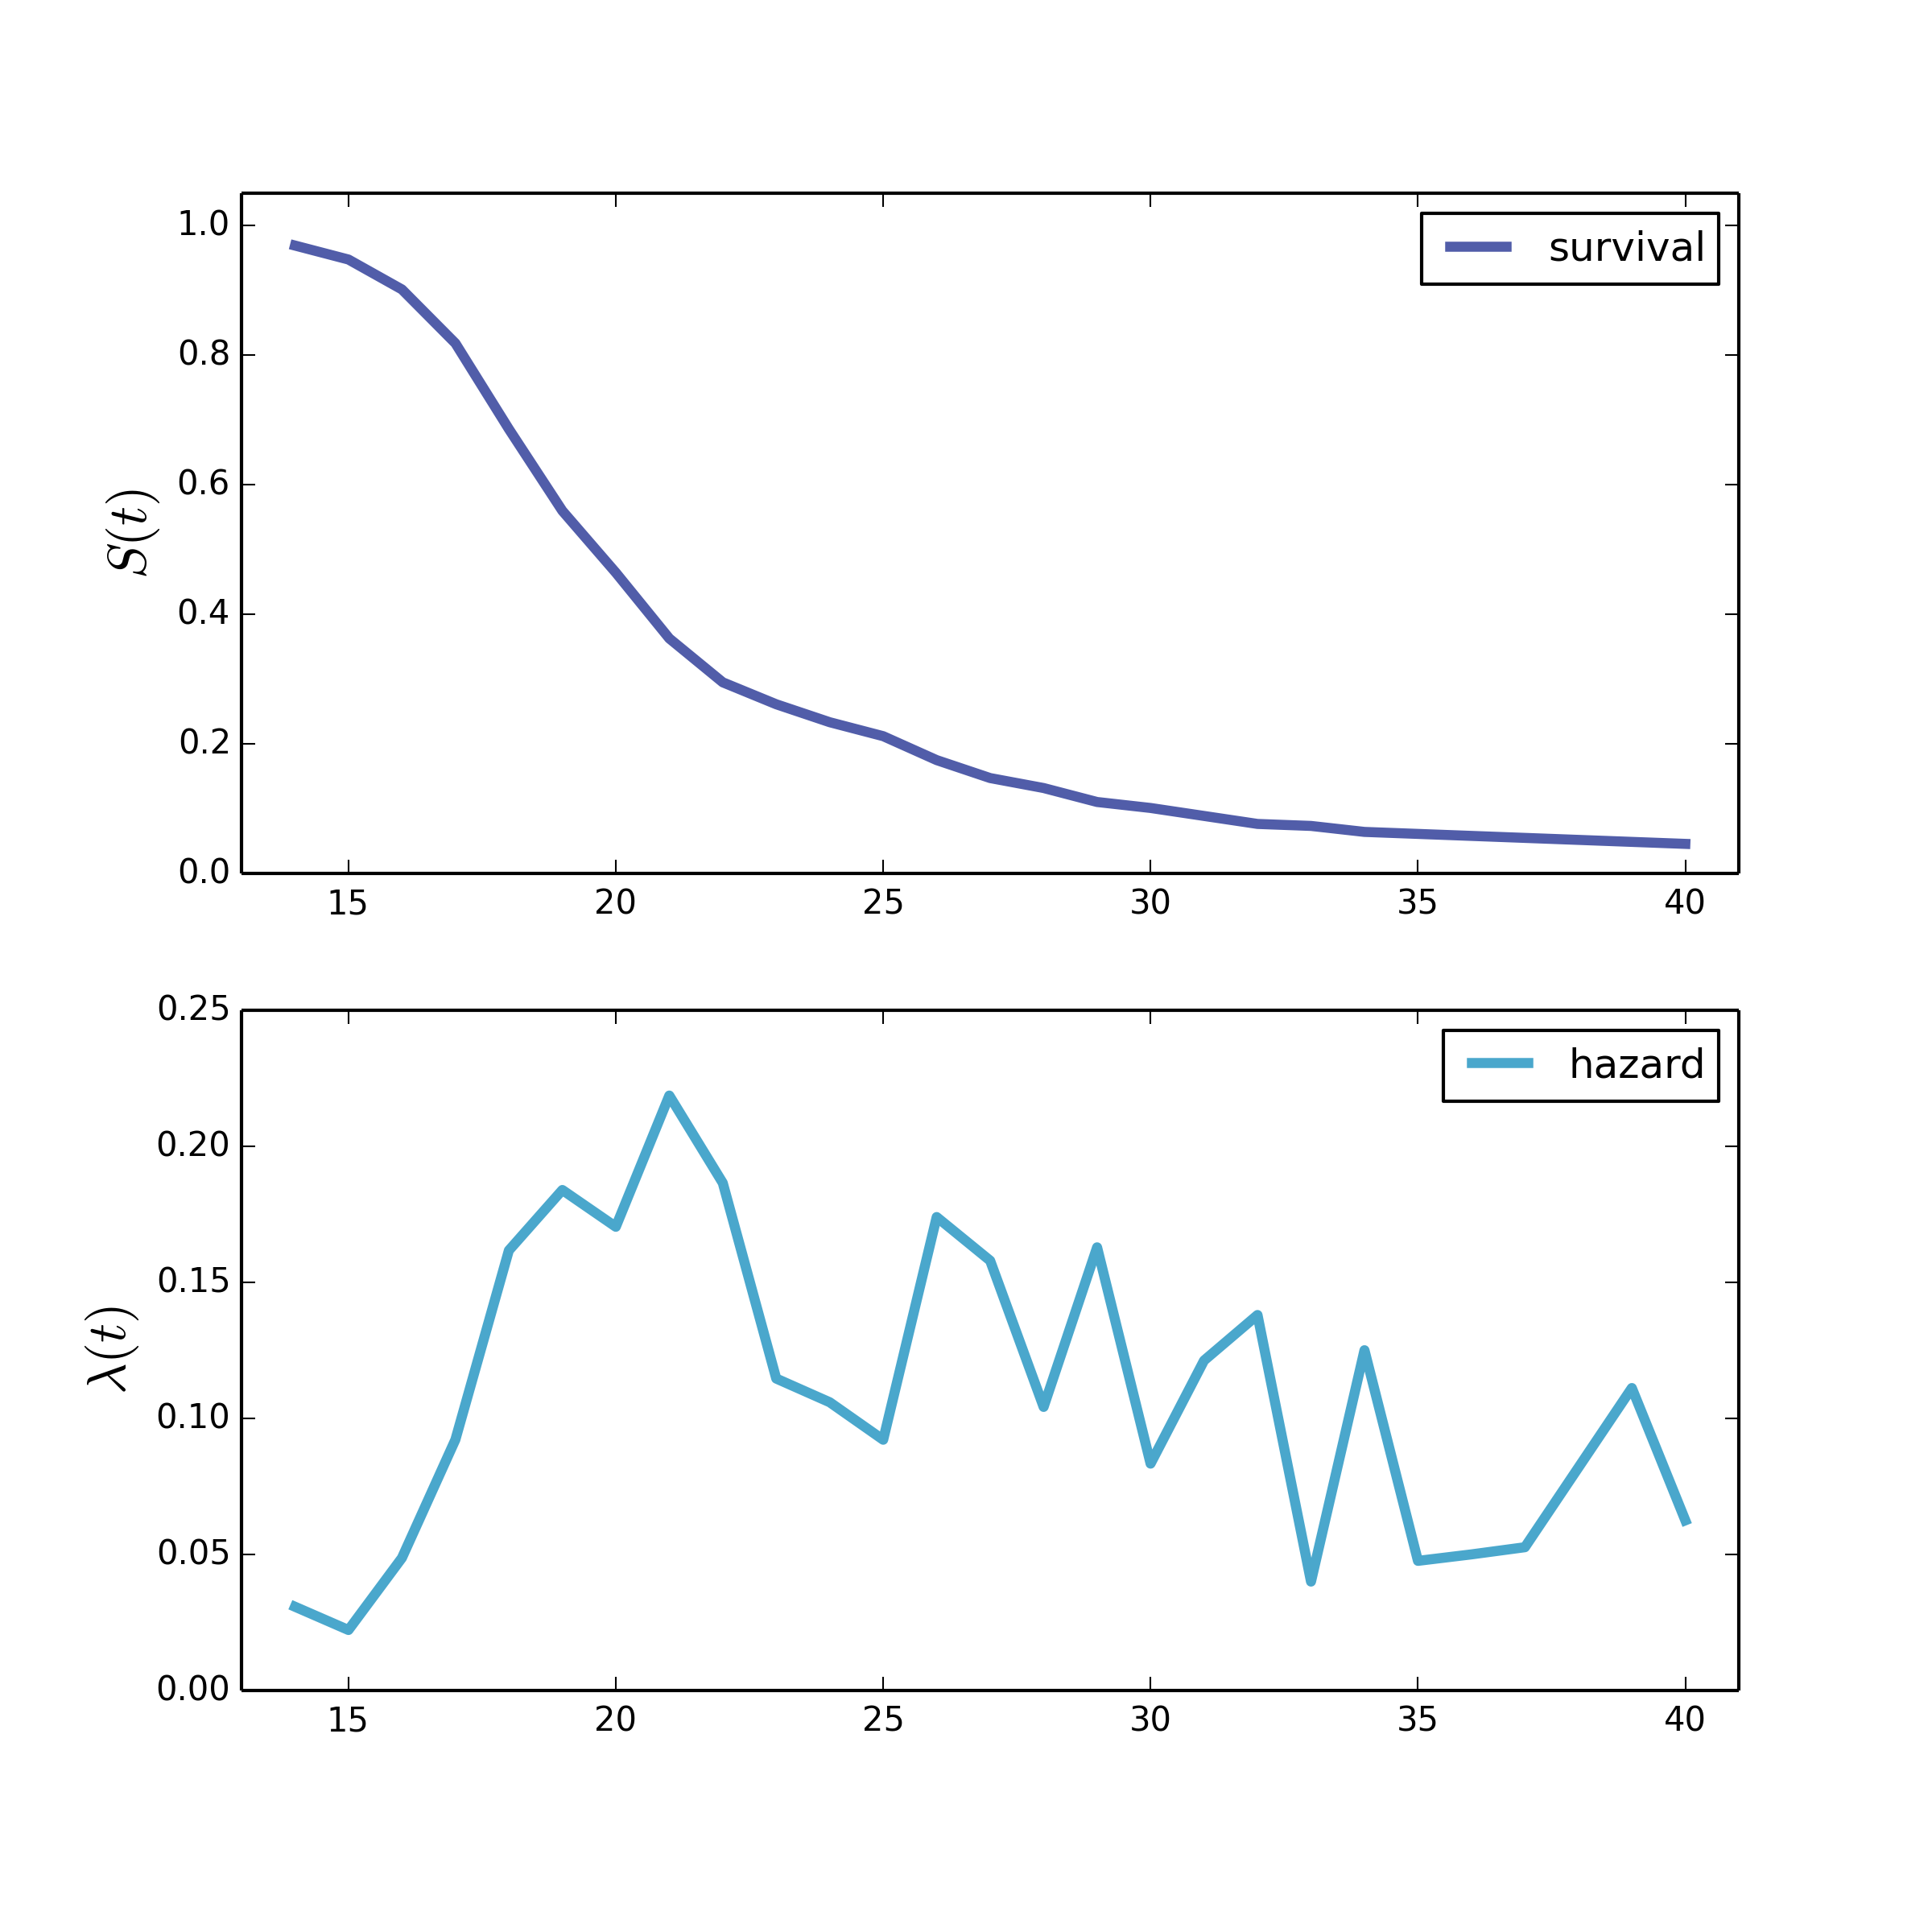
\includegraphics[width=3.75in]{marriage1}
\caption{Survival and hazard functions for 1930s cohort.}
\label{fig:marriage1}
\end{figure}

Figure~\ref{fig:marriage1} shows the survival and hazard functions
for women born in the 1930s.  These women were interviewed when they
were 42--44 years old.  At that point more than 95\% of them had been
married; for the others we set age at marriage to infinity ({\tt np.inf}).
In this cohort, the hazard function is highest at ages 18--22, and
lower as age increases.

This example demonstrates the simple case, where the respondents
are the same age and most events are complete.  But for most
applications of survival analysis, the sample also includes
incomplete events.  For example, the 1960s cohort includes women
from ages 14--44; for the ones that are not married, we don't know
when they will marry, if ever.  These missing data are said
to be ``censored''.

It might be tempting to ignore unmarried women and compute the
survival function for women whose ages at marriage are known.  But
that would discard useful information and seriously bias
the results.

For women who are not married yet, their age
at interview is a lower bound on their age at
marriage.  We can use both groups to estimate the hazard function,
then compute the survival function.  One common way to do
that is Kaplan-Meier estimation (see \url{https://en.wikipedia.org/wiki/Kaplan-Meier_estimator}).

The fundamental idea is that at each time, $t$, we know the number
of events that occurred and the number of respondents who were
``at risk''; that is, known to to be unmarried.  The ratio of these
factors estimates the hazard function.

Initially, the entire sample is considered at risk.  At each
time step, we subtract people who got married at age $t$ as well
as people who were interviewed at age $t$ (and therefore no
longer in the observation pool at the next time step).  The
following function implements this algorithm:

\begin{verbatim}
def EstimateHazard(complete, ongoing):
    hist_complete = Counter(complete)
    hist_ongoing = Counter(ongoing)

    ts = list(hist_complete|hist_ongoing)
    ts.sort()

    at_risk = len(complete)+len(ongoing)

    lams = pd.Series(index=ts)
    for t in ts:
        ended = hist_complete[t]
        censored = hist_ongoing[t]

        lams[t] = ended / at_risk
        at_risk -= ended + censored

    return HazardFunction(lams)
\end{verbatim}

{\tt complete} is a sequence of lifetimes for complete events,
in this case age at marriage.  {\tt ongoing} is a sequence of
lower bounds for incomplete observations, in this case age at
interview.

\verb"hist_complete" counts how many respondents were married
at each age; \verb"hist_ongoing" counts how many unmarried
respondents were interviewed at each age.

{\tt ts} is a sorted list of observation times, which is the
union of unique values from {\tt complete} and {\tt ongoing}.

\verb"at_risk" is the number of respondents at risk; initially
it is the total number of respondents.

{\tt lams} is a Pandas Series that maps from each observation
time to the estimated hazard rate.  

For each value of {\tt t} we compute {\tt ended}, which is
the number of people married at {\tt t}, and {\tt censored}, which
is the number of people interviewed at {\tt t}.  The hazard
function at {\tt t} is just the ratio of {\tt ended} and
\verb"at_risk".

At the end of each time step, we subtract {\tt ended} and
{\tt censored} from \verb"at_risk".

The result is a HazardFunction object that contains the Series
{\tt lams} and provides methods to access it.

With this estimated HazardFunction, we can compute the SurvivalFunction.
The hazard function, $\lambda(t)$, is the probability of ending at time $t$
conditioned on surviving until $t$.  Therefore, the probability
of surviving until $t$ is the cumulative product
of the complementary hazard function:
%
\begin{equation}
S(t) = \prod_{t_i < t} \left[1 - \lambda(t_i)\right]
\end{equation}
%
Here's the Python implementation:

\begin{verbatim}
# class HazardFunction
def MakeSurvival(self):
    series = (1 - self.series).cumprod()
    ts = series.index.values
    ss = series.values
    return SurvivalFunction(ts, ss)
\end{verbatim}

We wrote our own implementation of these methods in
order to demonstrate the methodology, and also to make them
work efficiently with the
resampling methods described in the next section.  But
Kaplan-Meier estimation and other survival analysis algorithms
are also implemented in a Python package called Lifelines
(see \url{http://lifelines.readthedocs.org}).


\subsection{Resampling}

The NSFG is intended to be representative of the adult U.S.\ population,
but it uses stratified sampling to systematically oversample certain
subpopulations, including teenagers and racial minorities.  Our analysis
takes this design into account to generate results that are
representative of the population.

As an example of stratified sampling, 
suppose there are 10 000 people in the population you are studying, and
you sample 100.  Each person in the sample represents 100 people in the
population, so each respondent has the same ``sampling weight''.

Now suppose there are two subgroups, a minority of 1 000 people and a 
majority of 9 000.  A sample of 100 people will have 10 members of the
minority group, on average, which might not be enough for reliable
statistical inference.

In a stratified sample, you might survey 40 people from the minority
group and only 60 from the majority group.  This design improves the power
of the sample, but it changes the weight associated with each respondent.
Each of the 40 minorities represents $1000 / 40 = 25$ people in the
population, while each of the 60 others represents $9000 / 60 = 150$ people.
In general, respondents from oversampled
groups have lower weights.

The NSFG includes a computed weight for each respondent that indicates
how many people in the U.S.\ population she represents.  
Some statistical methods, like regression, can be extended to take these
weights into account, but in general it is not easy.

However, bootstrapping provides a simple and effective approach.
The idea behind bootstrapping is to use the actual sample as a model of
the population, then simulate the results of additional experiments
by drawing new samples (with replacement) from the actual sample.

With stratified sampling, we can modify the bootstrap process to take sampling
weights into account.  The following function performs weighted resampling
on the NSFG data:

\begin{verbatim}
def ResampleRowsWeighted(df):
    weights = df.finalwgt
    cdf = thinkstats2.Cdf(dict(weights))
    indices = cdf.Sample(len(weights))
    sample = df.loc[indices]
    return sample
\end{verbatim}

{\tt df} is a Pandas DataFrame with one row per respondent and a column
that contains sampling weights, called {\tt finalwgt}.

{\tt weights} is a Series that maps
from respondent index to sampling weight.  {\tt cdf} represents a
cumulative distribution function that maps from each index to
its cumulative probability.  The Cdf class is provided by 
{\tt thinkstats2}, a Python module that accompanies the second
edition of {\it Think Stats}\cite{downey14}.

{\tt Sample} generates a random sample of indices based on the
sampling weights.  The return value, {\tt sample}, is a Pandas
DataFrame that contains the selected rows.
Since the sample is generated with replacement, some respondents might appear
more than once; others might not appear at all.

After resampling, we jitter the data by adding Gaussian noise (mean 0, standard
deviation 1 year) to the respondents' age at interview and age at marriage.
Jittering contributes some smoothing, which
makes the figures easier to interpret, and some robustness, making the
results less prone to the effect of a small number of idiosyncratic 
data points.

Jittering makes sense in the context of bootstrapping: each respondent in
the sample represents several thousand people in the population.  It is
reasonable to assume that there is variation within each represented
subgroup.

Finally, we discretize age at interview and age at marriage, rounding down
to integer values.


\section{Results}

\begin{figure}[!t]
\centering
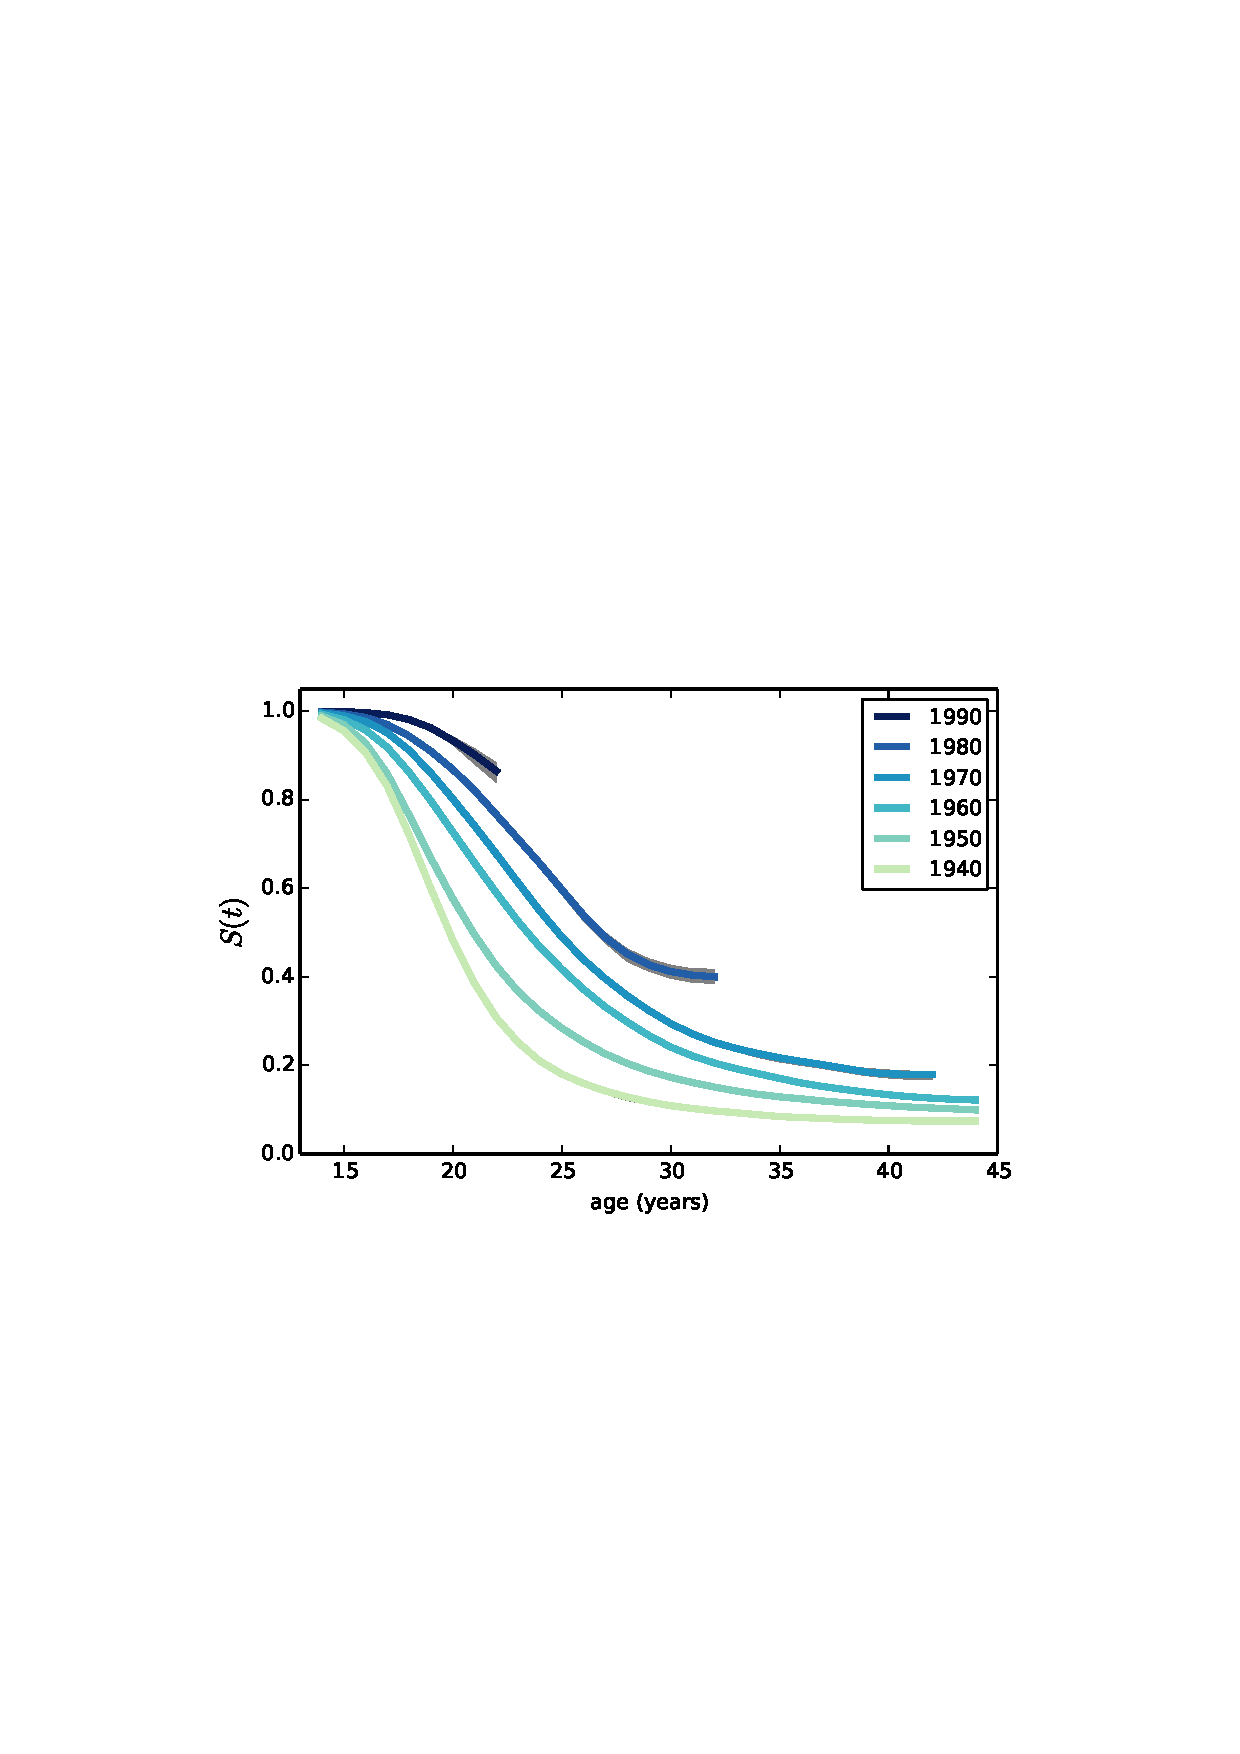
\includegraphics[width=3.75in]{marriage2}
\caption{Survival functions.}
\label{fig:marriage2}
\end{figure}

Figure~\ref{fig:marriage2} shows the estimated survival curve for each
cohort (we omit the 1930s cohort because it only includes people born
after 1936, so it is not representative of the decade).  The colored
lines show the median of 101 resampling runs; the gray regions show
90\% confidence intervals.

Two trends are apparent in this figure: women are getting married
later, and the fraction of women who remain unmarried is increasing.

Table~\ref{tab:cohorts2} shows the percentage of married women
in each cohort at ages 22, 32, and 42 (which are the last observed
ages for cohorts 90, 80, and 70).

\begin{table}[ht]
\centering
\begin{tabular}{c|r|r|r}
Cohort & \multicolumn{3}{c}{\% married by age} \\
       & 22  & 32  & 42 \\
\hline
40 & 69 & 90 & 92 \\
50 & 57 & 85 & 90 \\
60 & 41 & 79 & 87 \\
70 & 32 & 75 & 82 \\
80 & 23 & 60 & -- \\
90 & 13 & -- & -- \\
\end{tabular}
\caption{Marriage rates by birth cohort and age.}
\label{tab:cohorts2}
\end{table}

Two features of this data are striking:

\begin{itemize}
\item At age 22, only 13\% of
the 90s cohort have been married, contrasted with 69\% of the 40s cohort.
Between these cohorts, the fraction of women married by age 22
has dropped more than 11 percentage points per decade.

\item At age 32, only 60\% of the 80s cohort is married, and
their survival curve seems to have gone flat.  In this cohort,
259 were at risk at age 30, and only 9 were married that year;
155 were at risk at age 31, and none were married;
63 were are risk at age 32, and again none were married.
These low hazard rates are strange, but they are based on
sample sizes large enough that it is hard to dismiss them.

\end{itemize}


\subsection{Projection}

Predicting these kinds of social trends is
nearly futile.  As we saw in the previous section, the
80s cohort seems to be on strike, with unprecedented low marriage
rates in their early thirties.  Simple extrapolation of their
survival curve predicts that 40\% of them will remain unmarried,
more than double the fraction of previous generations.

But at the same time the fraction of women getting married at
ages 35--45 has been increasing for several generations, so we
might expect that trend to continue.  In that case the gap between
the 80s and 70s cohorts might close.

These prediction methods yield contradictory results.  A
simple middle ground is to assume that the hazard function from
the previous generation will apply to the next.  For example,
for the 70s cohort, the hazard rate at age 33 was 4.6\%.  In
the 80s cohort, there will be 14 women at risk at age 33, so
we predict that $0.64$ of them will get married.

To make these projections (and avoid the word ``prediction''),
we extend each HazardFunction using
data from the previous cohort:

\begin{verbatim}
# class HazardFunction
def Extend(self, other):
    last_t = self.series.index[-1]
    other_ts = other.series.index
    hs = other.series[other_ts > last_t]
    seq = self.series, hs
    self.series = pd.concat(seq)
\end{verbatim}

Then we convert the extended hazard functions to survival functions,
using {\tt HazardFunction.MakeSurvival}.

\begin{figure}[!t]
\centering
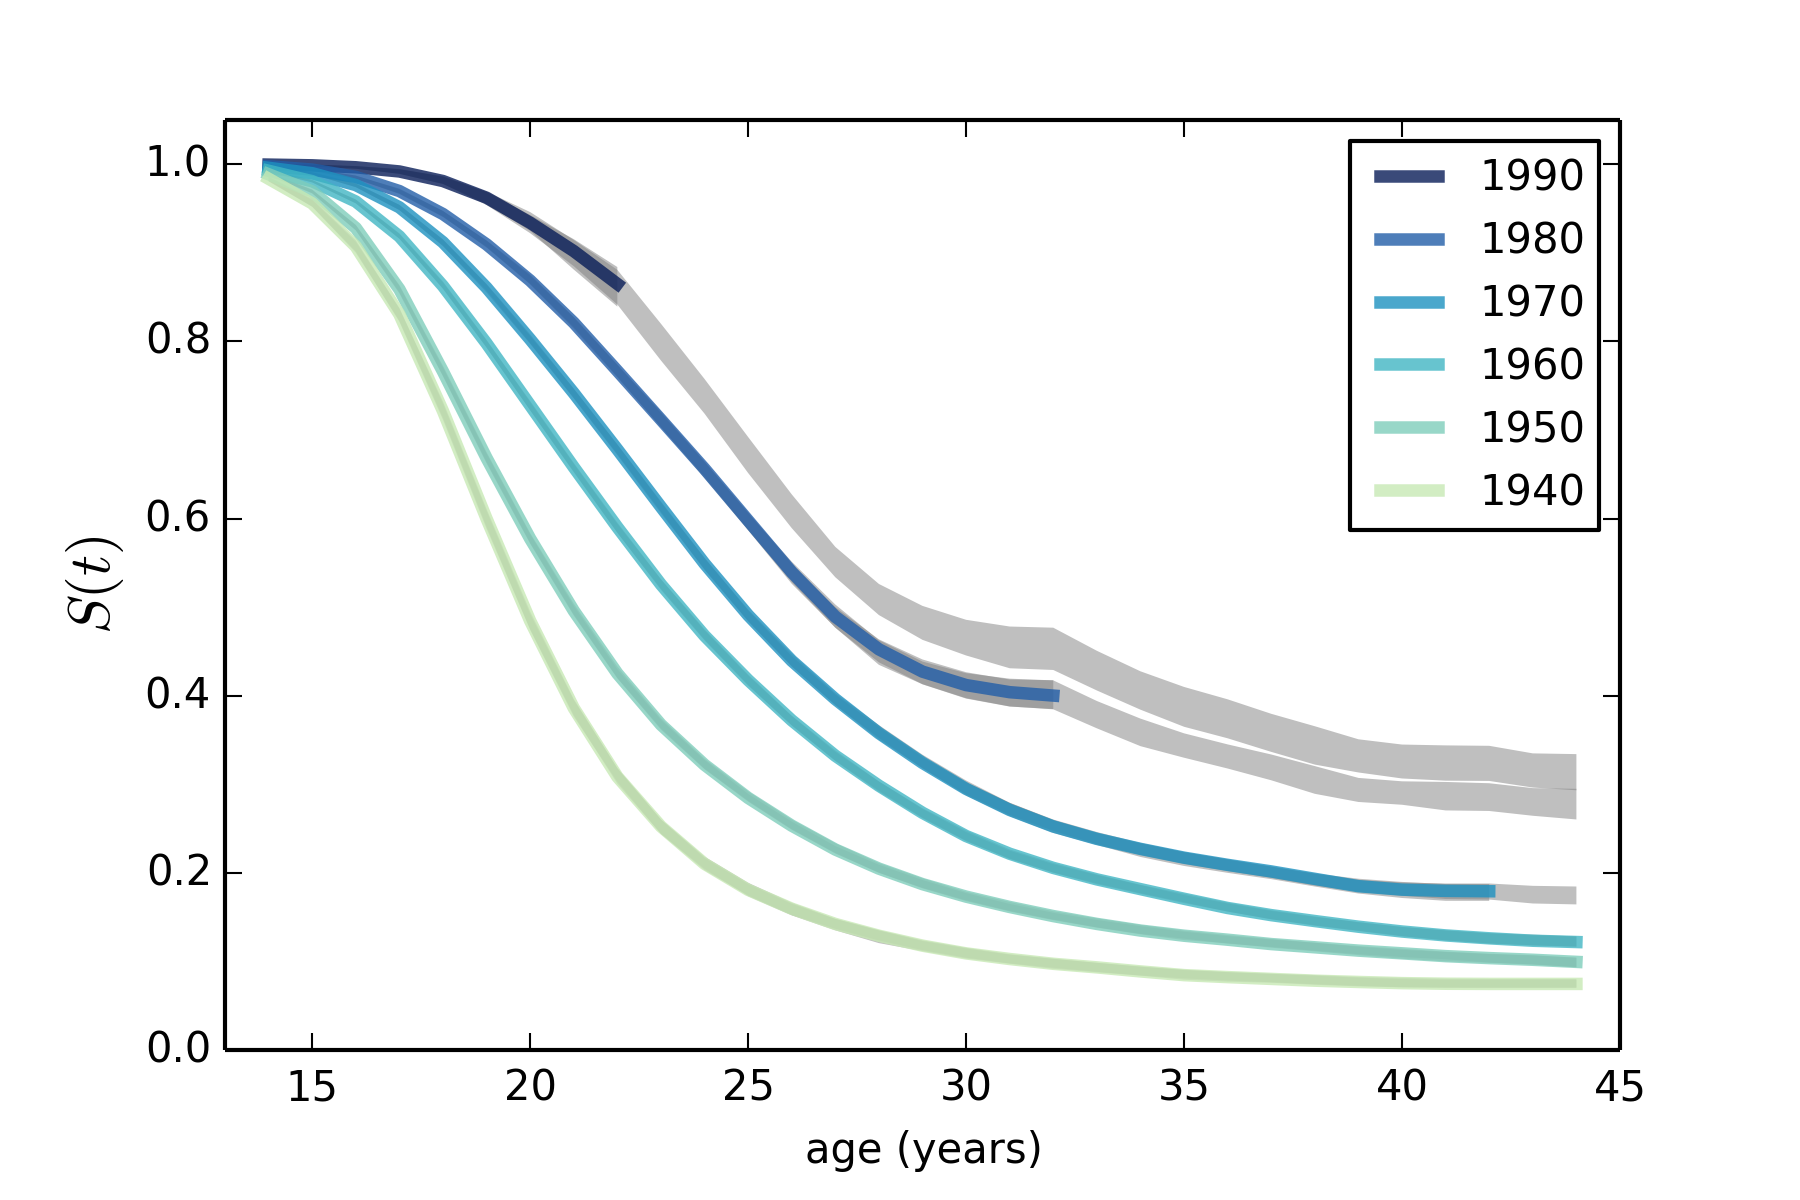
\includegraphics[width=3.75in]{marriage3}
\caption{Survival functions with projections.}
\label{fig:marriage3}
\end{figure}

Figure~\ref{fig:marriage3} shows the results.  Again,
the gray regions show a 90\% confidence interval.  For
the 80s cohort, the median projection is that 72\% will marry by
age 44, down from 82\% in the previous cohort.

For the 90s cohort, the median projection is that only 68\% will
marry by age 44.  But the projection assumes that this cohort will
also go on a ``marriage strike'' in their early thirties.
This event is probably
idiosyncratic and unlikely to be repeated.  So, again, we should
not take these predictions too seriously.


\section{Future work}

This work is preliminary, and there are many avenues for future
investigation:

\begin{itemize}

\item The NSFG includes data from male respondents, starting with Cycle 6
in 2002.  We plan to repeat our analysis for male respondents.

\item There are many subgroups in the U.S.\ that would be
interesting to explore, including different regions, education
and income levels, racial and religious groups. 

\item We have data from the Canadian General Social Survey,
which will allow us to compare marriage patterns between countries
(see \url{http://tinyurl.com/canadagss}).

\item We are interested in finding similar data from other countries.

\end{itemize}


% use section* for acknowledgement
\section*{Acknowledgment}
Many thanks to Lindsey Vanderlyn for help with data acquisition,
preparation, and analysis.


% Can use something like this to put references on a page
% by themselves when using endfloat and the captionsoff option.
\ifCLASSOPTIONcaptionsoff
  \newpage
\fi




\begin{thebibliography}{1}

\bibitem{downey14}
Allen Downey, {\it Think Stats: Exploratory Data Analysis}", 2nd edition, 
            O'Reilly Media, October 2014.
            \url{http://thinkstats2.com}

\bibitem{wang14}
Wendy Wang and Kim Parker, "Record Share of Americans 
           Have Never Married", Washington D.C.: Pew Research Center's
           Social and Demographic Trends project, September 2014.
           \url{http://tinyurl.com/wang14pew}
           

\end{thebibliography}



\begin{IEEEbiography}[{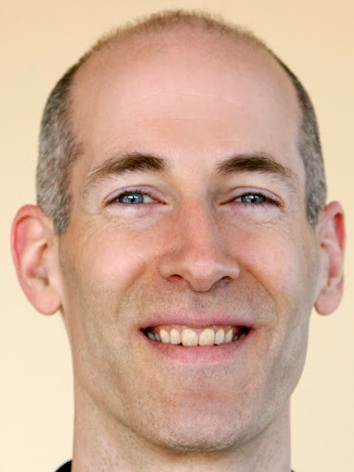
\includegraphics[width=1in,height=1.25in,clip,keepaspectratio]{allen_downey}}]{Allen B. Downey}
is a Professor of Computer Science at Olin College of Engineering
in Needham MA, where he teaches programming, data science, and scientific computing.
He is the author of several free textbooks, including
{\it Think Bayes}, {\it Think Stats}, and {\it Think Python}, all published
by O'Reilly Media and available from Green Tea Press: \url{http://greenteapress.com}.  He offers workshops and consults on data
science and Bayesian statistics.
\end{IEEEbiography}


\end{document}


